%=======================02-713 LaTeX template, following the 15-210 template==================
%
% You don't need to use LaTeX or this template, but you must turn your homework in as
% a typeset PDF somehow.
%
% How to use:
%    1. Update your information in section "A" below
%    2. Write your answers in section "B" below. Precede answers for all 
%       parts of a question with the command "\question{n}{desc}" where n is
%       the question number and "desc" is a short, one-line description of 
%       the problem. There is no need to restate the problem.
%    3. If a question has multiple parts, precede the answer to part x with the
%       command "\part{x}".
%    4. If a problem asks you to design an algorithm, use the commands
%       \algorithm, \correctness, \runtime to precede your discussion of the 
%       description of the algorithm, its correctness, and its running time, respectively.
%    5. You can include graphics by using the command \includegraphics{FILENAME}
%
\documentclass[11pt]{article}
\usepackage{amsmath,amssymb,amsthm}
\usepackage{graphicx}
\usepackage[margin=1in]{geometry}
\usepackage{fancyhdr}
\usepackage{listings}
\setlength{\parindent}{0pt}
\setlength{\parskip}{5pt plus 1pt}
\setlength{\headheight}{13.6pt}
\newcommand\question[2]{\vspace{.25in}\hrule\textbf{#1: #2}\vspace{.5em}\hrule\vspace{.10in}}
\renewcommand\part[1]{\vspace{.10in}\textbf{(#1)}}
\newcommand\algorithm{\vspace{.10in}\textbf{Algorithm: }}
\newcommand\ot{\vspace{.10in}\textbf{Output: }}
\newcommand\runtime{\vspace{.10in}\textbf{Running time: }}
\pagestyle{fancyplain}
\lhead{\textbf{\NAME\ (\ANDREWID)}}
\chead{\textbf{Lab\HWNUM}}
\rhead{\today}
\begin{document}\raggedright
%Section A==============Change the values below to match your information==================
\newcommand\NAME{Yao Xiao}  % your name
\newcommand\ANDREWID{2019180015}     % your andrew id
\newcommand\HWNUM{6}              % the homework number
%Section B==============Put your answers to the questions below here=======================

% no need to restate the problem --- the graders know which problem is which,
% but replacing "The First Problem" with a short phrase will help you remember
% which problem this is when you read over your homeworks to study.

\question{1}{The First Problem} 

\part{a} \algorithm
\begin{lstlisting}
import math
import numpy as np

def cal_dist(point1: np.ndarray, point2: list) -> float:
    distance = 0.0
    for a, b in zip(point1, point2):
        distance += math.pow(a - b, 2)
    return math.sqrt(distance)


class Node(object):
    def __init__(self,
                 cent,
                 left=None,
                 right=None,
                 distance=-1,
                 tag=None,
                 count=1):
        self.cent = cent
        self.left = left
        self.right = right
        self.distance = distance
        # tag calculated node
        self.tag = tag
        self.count = count


class AC(object):
    def __init__(self, k=1):
        assert k > 0
        self.k = k
        self.labels = None

    def fit(self, x):
        nodes = [Node(cent=v, tag=i) for i, v in enumerate(x)]
        distances = {}
        point_num, future_num = np.shape(x)
        self.labels = [-1] * point_num
        current_tag = -1
        while len(nodes) > self.k:
            min_dist = math.inf
            nodes_len = len(nodes)
            closest_part = None
            for i in range(nodes_len - 1):
                for j in range(i + 1, nodes_len):
                    d_key = (nodes[i].tag, nodes[j].tag)
                    if d_key not in distances:
                        distances[d_key] = cal_dist(nodes[i].cent,
                                                    nodes[j].cent)
                    d = distances[d_key]
                    if d < min_dist:
                        min_dist = d
                        closest_part = (i, j)
            # merge
            part1, part2 = closest_part
            node1, node2 = nodes[part1], nodes[part2]
            new_cent = [
                (node1.cent[i] * node1.count + node2.cent[i] * node2.count) /
                (node1.count + node2.count) for i in range(future_num)
            ]
            new_node = Node(cent=new_cent,
                            left=node1,
                            right=node2,
                            distance=min_dist,
                            tag=current_tag,
                            count=node1.count + node2.count)
            current_tag -= 1
            del nodes[part2], nodes[part1]
            nodes.append(new_node)
        self.nodes = nodes
        self.cal_label()

    def cal_label(self):
        for i, node in enumerate(self.nodes):
            self.order(node, i)

    def order(self, node: Node, label):
        if node.left is None and node.right is None:
            self.labels[node.tag] = label
        if node.left:
            self.order(node.left, label)
        if node.right:
            self.order(node.right, label)
\end{lstlisting}


\question{2}{The Second Problem}
\part{a} \algorithm
\begin{lstlisting}
from sklearn import datasets
from sklearn import cluster

iris = datasets.load_iris()
ac = AC(4)
ac.fit(iris.data)
print(np.array(ac.labels))

sk = cluster.AgglomerativeClustering(4)
sk.fit(iris.data)
print(sk.labels_)
\end{lstlisting}

\part{b} \ot Self-implemented AC algorithm VS AgglomerativeClustering from sklearn\\
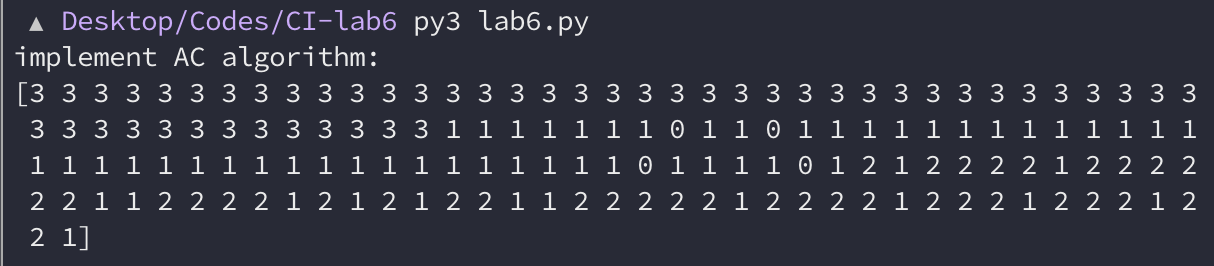
\includegraphics[scale=0.8]{f1.png}
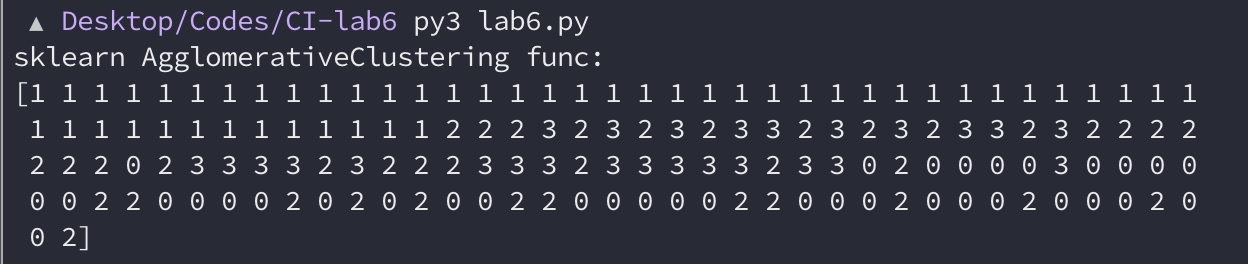
\includegraphics[scale=0.78]{f2.png}

\end{document}
